%---=---==---===---====---=====---======---=====---====---===---==---=---%
%-         REQUIREMENTS ANALYSIS AND REQUIREMENTS SPECIFICATION         -%
%---=---==---===---====---=====---======---=====---====---===---==---=---%

\chapter{Requirements}\label{chap:requirements}

This chapter focuses on project requirements. It begins with an explanation of the process of requirements \nameandsecref{sec:requirementscapture} and analysis, continues with a discussion of crucial \nameandsecref{sec:requirements} and areas of particular challenge, and then ends with addressing, with prudence, the issue of project \nameandsecref{sec:scope}.

\section{Capture} \label{sec:requirementscapture}

Requirements are an essential aspect of any project, as they formulate the purpose of the software, and set clear goals. Without requirements, developers may lose sight of what needs completing, and so may fail to deliver as expected; it would also cause problems in testing, as testers would be unable to refer to how an application should function. A keen effort was made to develop specific requirements, with low ambiguity, and written concisely.

In this project, the requirements were captured from the \nameandsecref{chap:background}, through research and technology review. Relevant academic papers were evaluated to ascertain what is possible to develop using current state-of-the-art methods, and these are reflected on in the requirements. Also, technology was reviewed to determine what had gone well, not so well, and what to avoid doing from previous projects.

Another method used for requirements capture was the short coding exercise in \cref{subsec:hough}, which was key to the capture process. Short coding can quickly validate a method before allotting it a more substantial amount of time, in this case, time was saved by determining that using markerless detection methods; specifically, the Hough-Lines transform, was infeasible.

\section{Requirements} \label{sec:requirements}

Using the techniques discussed previously in \cref{sec:requirementscapture}, this section aims to formulate requirements in response to the problems identified in \cref{sec:challenges}. It opens a discussion into the critical requirements in each stage of the system, explains why they were chosen and focuses on areas of particular challenge, difficulty or conflict. The full breakdown of requirements can be found in \cref{app:requirements}.

\subsection{\detection}



As was summarised in \cref{subsec:detectionsummary}, the system should use marker-based detection methods because of its clear advantages over markerless detection. Namely, it allows for an immediate understanding of object poses without the need for further analysis. Another reason to use marker based detection is that if a marker is detected, then it is known that a block exists at that location, meaning that it implicitly meets \cref{req:blocknonblock,req:tower}, which would otherwise require explicit solving.

Moreover, UcoSLAM is a library well fit for this project, due to its ability to map the locations of both markers and key points, thus gaining a deeper understanding of the environment, and so it should be adopted as the method of choice.

\subsubsection{Pose Estimation}\label{subsec:poseestimation}

There are a few options to consider for how to employ marker-based detection with a \jenga{} tower, in particular, answering the question of which block faces should markers be affixed. Firstly, affixing markers to every face would be a viable solution, as it means every block face can be identified and have its pose estimated; however, this solution involves a high setup time cost, and it also requires a larger dictionary of markers. Using a larger dictionary is disadvantageous because it means that the detection algorithm needs to search for more markers, thus increasing detection time, and also resulting in a higher chance for errors, i.e. false positives \citep{ucoslampaper}.

The opposite of the above solution is only to use one marker per block, which is better because it has less setup time, and requires a smaller dictionary size. If a single marker is attached to an end face of a block, then after estimating its pose, the full block pose can be estimated by using known dimensions, which in the official game are 15mm x 25mm x 75mm. On first look, this solution seems like it would be successful, although the faces are small, and markers will have to be even smaller, as there needs to be a relatively small amount of whitespace around each marker so that the detection algorithm does not confuse multiple markers as being part of one. Also, small markers are subject to pose ambiguity, as shown in \cref{fig:poseambiguity}, so although a marker pose estimations may be incorrect.

\begin{figure}[ht]
\begin{minipage}{\textwidth}
    \centering
    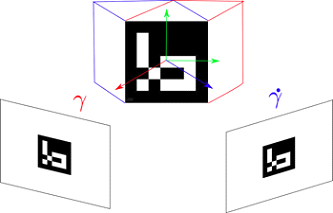
\includegraphics{images/requirements/ambiguity_problem.png}
    \caption{The ambiguity problem, image from the \protect\footurl{https://docs.google.com/document/d/1QU9KoBtjSM2kF6ITOjQ76xqL7H0TEtXriJX5kwi9Kgc}{ArUco Documentation}}
    \label{fig:poseambiguity}
\end{minipage}
\end{figure}

The ArUco library tries to solve the ambiguity itself, by using various error correction methods, but there is a way to can solve the ambiguity problem with \jenga{} pieces; that is affixing a marker to both end faces of each block. This eliminates the problem by estimating the position and orientation of both markers for a tower piece, and then reconstructing the piece to be between the two markers. In fact, this method means that the pose of each marker can be discarded, as only their relative locations are required for reconstruction.

\subsubsection{Camera}

A problem that comes with marker-based detection is camera distortion, which is common with modern cameras. Distortion is a problem because it means that two separate cameras could look at the same environment and come to a different understanding. As this project plans to solve the block removal problem in a real-world environment, as opposed to a lab-style fixed-camera environment as in previous solutions, this solution must account for camera-specific distortion, which brings about the need for \cref{req:camera}.

\begin{figure}[ht]
\begin{minipage}{\textwidth}
    \centering
    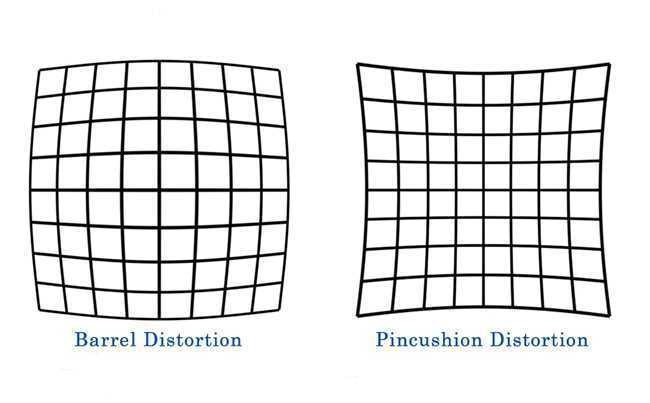
\includegraphics[width=.6\textwidth]{images/requirements/camera-distortion.jpg}
    \caption{Camera distortion, image from \protect\footurl{https://clickitupanotch.com/lens-distortion/}{Click it up a Notch}}
    \label{fig:cameradistortion}
\end{minipage}
\end{figure}

Another critical requirement is that the detection stage must be able to send the information it acquires about the block poses to the analysis stage, this is because a working system must have communication between its components; otherwise, it is not a single system, but a sum of separate components. Also, the stages may be written in different languages, so communication should be language independent. The requirements for the analysis stage are described next.

\subsection{\analysis}

\cref{sec:categoriessummary} identified that the most appropriate category for modelling a \jenga{} tower is parts-based. Marker-based detection compliments part-based modelling because a virtual block can easily be created between two markers, whereas other types of modelling would require more work to reach the same outcome.

\subsubsection{Reconstruction}
The marker map gained from the detection stage can be used to reconstruct the tower (\cref{req:reconstruct}), this needs to be done in such a way that the initial virtual tower remains stable if its real-world equivalent is also stable. However, there may be inaccuracies in the marker map, which presents the problem in physics simulations that some blocks may overlap when built solely from the positions in the marker map. To solve this, the system must account for pose estimation inaccuracies, which brings about \cref{req:inaccuracies}. It is worth noting that this would not be a problem with heuristic analysis because the analysis is less advanced and exact block poses are not required.

\subsubsection{Ranking}
In \cref{sec:problem}, it was introduced that the main problem faced by \jenga{} players is deciding which block to remove (\cref{req:rank}). This has been addressed in several papers, as researched in \cref{sec:structuralanalysis}, with some opting for a heuristic analysis, and others a physics analysis.

A heuristic analysis involves the creation of a set of rules which determine how likely is it for the tower to fall after removing a block. Applying such a rule set to a tower state is fast, and can therefore be performed in real time. While the rule set is unlikely to contain rules that users cannot think of themselves, this method provides an immediate analysis of all blocks (\cref{req:realtime}), which users cannot do. A significant drawback to this type of analysis is that it only takes into account a few physical constraints, such as pivoting, but misses more complex physics factors like weight distribution and friction.

On the other hand, physics simulation, if done correctly, can accurately represent a real-world tower in a virtual environment, accounting for several more physics factors than the heuristic approach. Using such an approach would therefore result in a more accurate analysis, which would be more beneficial to the user, however, it would also take more time. It is favourable to allow the user to choose between these two approaches (\cref{req:multianalysis}), as they both have advantages over the other.

\subsection{\display}

Following on from the analysis stage, it is vital for the system to display the analysis results (\cref{req:display}). This can be achieved in various ways, but as discussed in the \nameandsecref{sec:motivation}, there is significant market potential in augmented reality, and so the system should show the analysis using this technology.

\subsection{System}

Finally, there is a set of requirements for the system itself, two of which that are key are being easy to understand (\cref{req:understand}) and keeping the attention of the user (\cref{req:attention}), this is because if the user does not know how to use the system, or loses interest, then they are usually only one tap away from closing the application and doing something else.

Furthermore, there are high priority requirements which focus on how the software is to be written. For instance, \cref{req:selfcontained,req:modular} describe that the system should be self-contained, meaning the user should be kept within the system when using the different stages, but also modular, to keep these stages programmatically separate for the means of maintainability (\cref{req:maintainable}) and extensibility (\cref{req:extendable}).

\section{Scope}\label{sec:scope}

This project spans over about seven months and includes much research and planning, followed by designs and extensive implementation. Testing is also a requirement for the project, without which the viability of the system would be unconfirmed. With such a short amount of time to complete the project, it is important for the scope to be adequately defined.

Moreover, the possibilities for this project are limitless, as it can be expanded in almost every direction. For example, current state-of-the-art methods for the detection of block poses go into significant detail, and would require months of research and development find or improve upon alone. Yet, this is only one of the three main stages to be completed in this project, and time must be divided up fairly between them.

It would have been useful to incorporate machine learning into both the detection, as advanced object classification, and the analysis stage, as an advanced prediction method. The machine learning method has the potential to be both accurate, and fast, in the analysis of block removal feasibility, making it more favourable than the heuristic and physics simulation options. However, this method was descoped because, without prior experience with machine learning techniques, it had the potential to engulf the rest of the project.

Further, augmented reality is an ever-growing field in Computer Science, and so new techniques are often created, which can be a problem. For instance, the latest technologies may not be as stable or clear to use as the less recent, well-documented alternatives. Also, a difficult decision arises if part way through the project a new technique was released that would seem to solve a problem in a better way than the technology found during research, due to pressing time constraints.

UcoSLAM, the library that will be used for block detection, is so cutting edge in its field that the paper describing its approach was only released in February of this year. Deciding to use the library so late in the project was not straightforward because although it appeared to be able to solve the block detection problem, there would be little support with development. Changing the scope to include UcoSLAM also reduced the amount of time available for design and implementation, but was deemed necessary due to the functionality it provided.

\section{Summary}

To summarise, this section has defined the functional and non-functional requirements for each stage of the system, as well as the system as a whole. The next chapter uses these requirements as the basis for system design.